\documentclass{article}
\usepackage[top=1in, bottom=1.25in, left=1.05in, right=1.05in]{geometry}
\usepackage{amsmath,graphicx}

% Example definitions.
% --------------------
\def\x{{\mathbf x}}
\def\L{{\cal L}}

% Title.
% ------
\title{Investigation on Parallelization of Deep Neural Network Training using Multiple GPUs}
%
% Single address.
% ---------------
\author{Hang Su$^1$$^2$, Haoyu Chen$^1$, Nelson Morgan$^2$}
\date{}

\begin{document}
%\ninept
%
\maketitle
%
\begin{abstract}
In this paper we introduce Butterfly mixing to parallel training of deep neural networks (DNN). Parallelization is done
in a model averaging manner. Data is partitioned and distributed to different nodes for local model update, and
model averaging (reduce) is done every few minibatches. We compare several different reduce stratgies, including
all reduce, butterfly mixing, ring reduce and hopping ring reduce. We show that all these methods can effectively
speed up neural network training. On swithboard data, a xx times speed up is achieved using 16 gpus.

\end{abstract}
%
%
\section{Introduction}
\label{sec:intro}
Deep Neural Networks (DNN) has shown its effeciveness in several machine learning tasks, espencially in speech
recognition. The large model size and massive training examples make DNN a powerful model for classification. However,
these two factors also slow down the training procedure of DNNs.

Parallelization of DNN training has been a popular topic since the revive of neural networks. Several different strategies
have been proposed to tackle this problem. Multiple thread CPU parallelization and single CUDA GPU implementation are compared
in \cite{scanzio2010parallel,vesely2010parallel}, and they show that single GPU could beat 8 cores CPU by a factor of 2.

Optimality for parallelization of DNN training was analyzed in \cite{seide2014parallelizability}, and based on the analysis, 
a gradient quantization approach was proposed to minimize communication cost \cite{seide20141}.

DistBelief proposed in \cite{dean2012large} reports a speed up of 2.2x using 8 CPU coresthan using a
single machine.


Asynchronous SGD using multiple GPUs achieved a 3.2x speed-up on 4 GPUs \cite{zhang2013asynchronous}.

A pipeline training approach was propoased in \cite{chen2012pipelined} and a 3.3x speedup was achieved using 4 GPUs, but this
method does not scale beyond number of layers in the neural network.

A speedup of 6x to 14x was achieved using 16 GPUs on training convolutional neural networks \cite{coates2013deep}. In this approach,
each GPU is responsible for a partition of the neural network. This approach is more useful for image classification where 
local structure of the neural network could be exploited.

Distributed model averaging using CPUs is proposed in \cite{zhang2014improving},
and a further improvement is done using natural gradient \cite{povey2014parallel}.


Butterfly mixing was proposed in \cite{zhao2013butterfly} to interleave communication with computation.


\section{Data parallelization and Model Averging}
Gradient descent method is applied to train the DNN model even it's a non-convex optimization problem. Since the size of training data is large, batch training is applied to approximately compute the gradient for each iteration. Rougly, the larger batch size, the higher converge speed. However, the large batch size brings the computing time and memory usage problem. With using distributed system, the gradient can be computed at each node, communicate among all the nodes, and average recieved gradient at each update iteration. This method can compute the reduced gradient accurategly, but it requires heavy communication, since we need to communicate at each update iteration. \\

However, if the weight rather than gradient of weight is choosen to reduce and average, it is not necessary to communicate the weight at each iteration. Thus, in this project, we choose to communicate the weight for some fixed iterations steps. 
\section{Different Reduce Strategies}
In this section, the three data reduce strategies are introduced, which are all-reduce, butterfly mixing and ring/hopping rIng reduce.

\subsection{All-reduce}

All-reduce startegy collects the weights from all the nodes in the network. The communication is bounded by the bandwidth. Fig.~1 is an example of all-reduce with 4 nodes. After one node collects all the weights, it will average the weights and then boardcast it too all the nodes. Thus, the all-reduce requires at least twice communication to collect and boardcast the messages. However, the all-reduce can compute the average weight based on full information for the whole network. Thus, the converge speed of all-reduce should be the fastest.
\begin{figure}[h!]
  
  \centering
    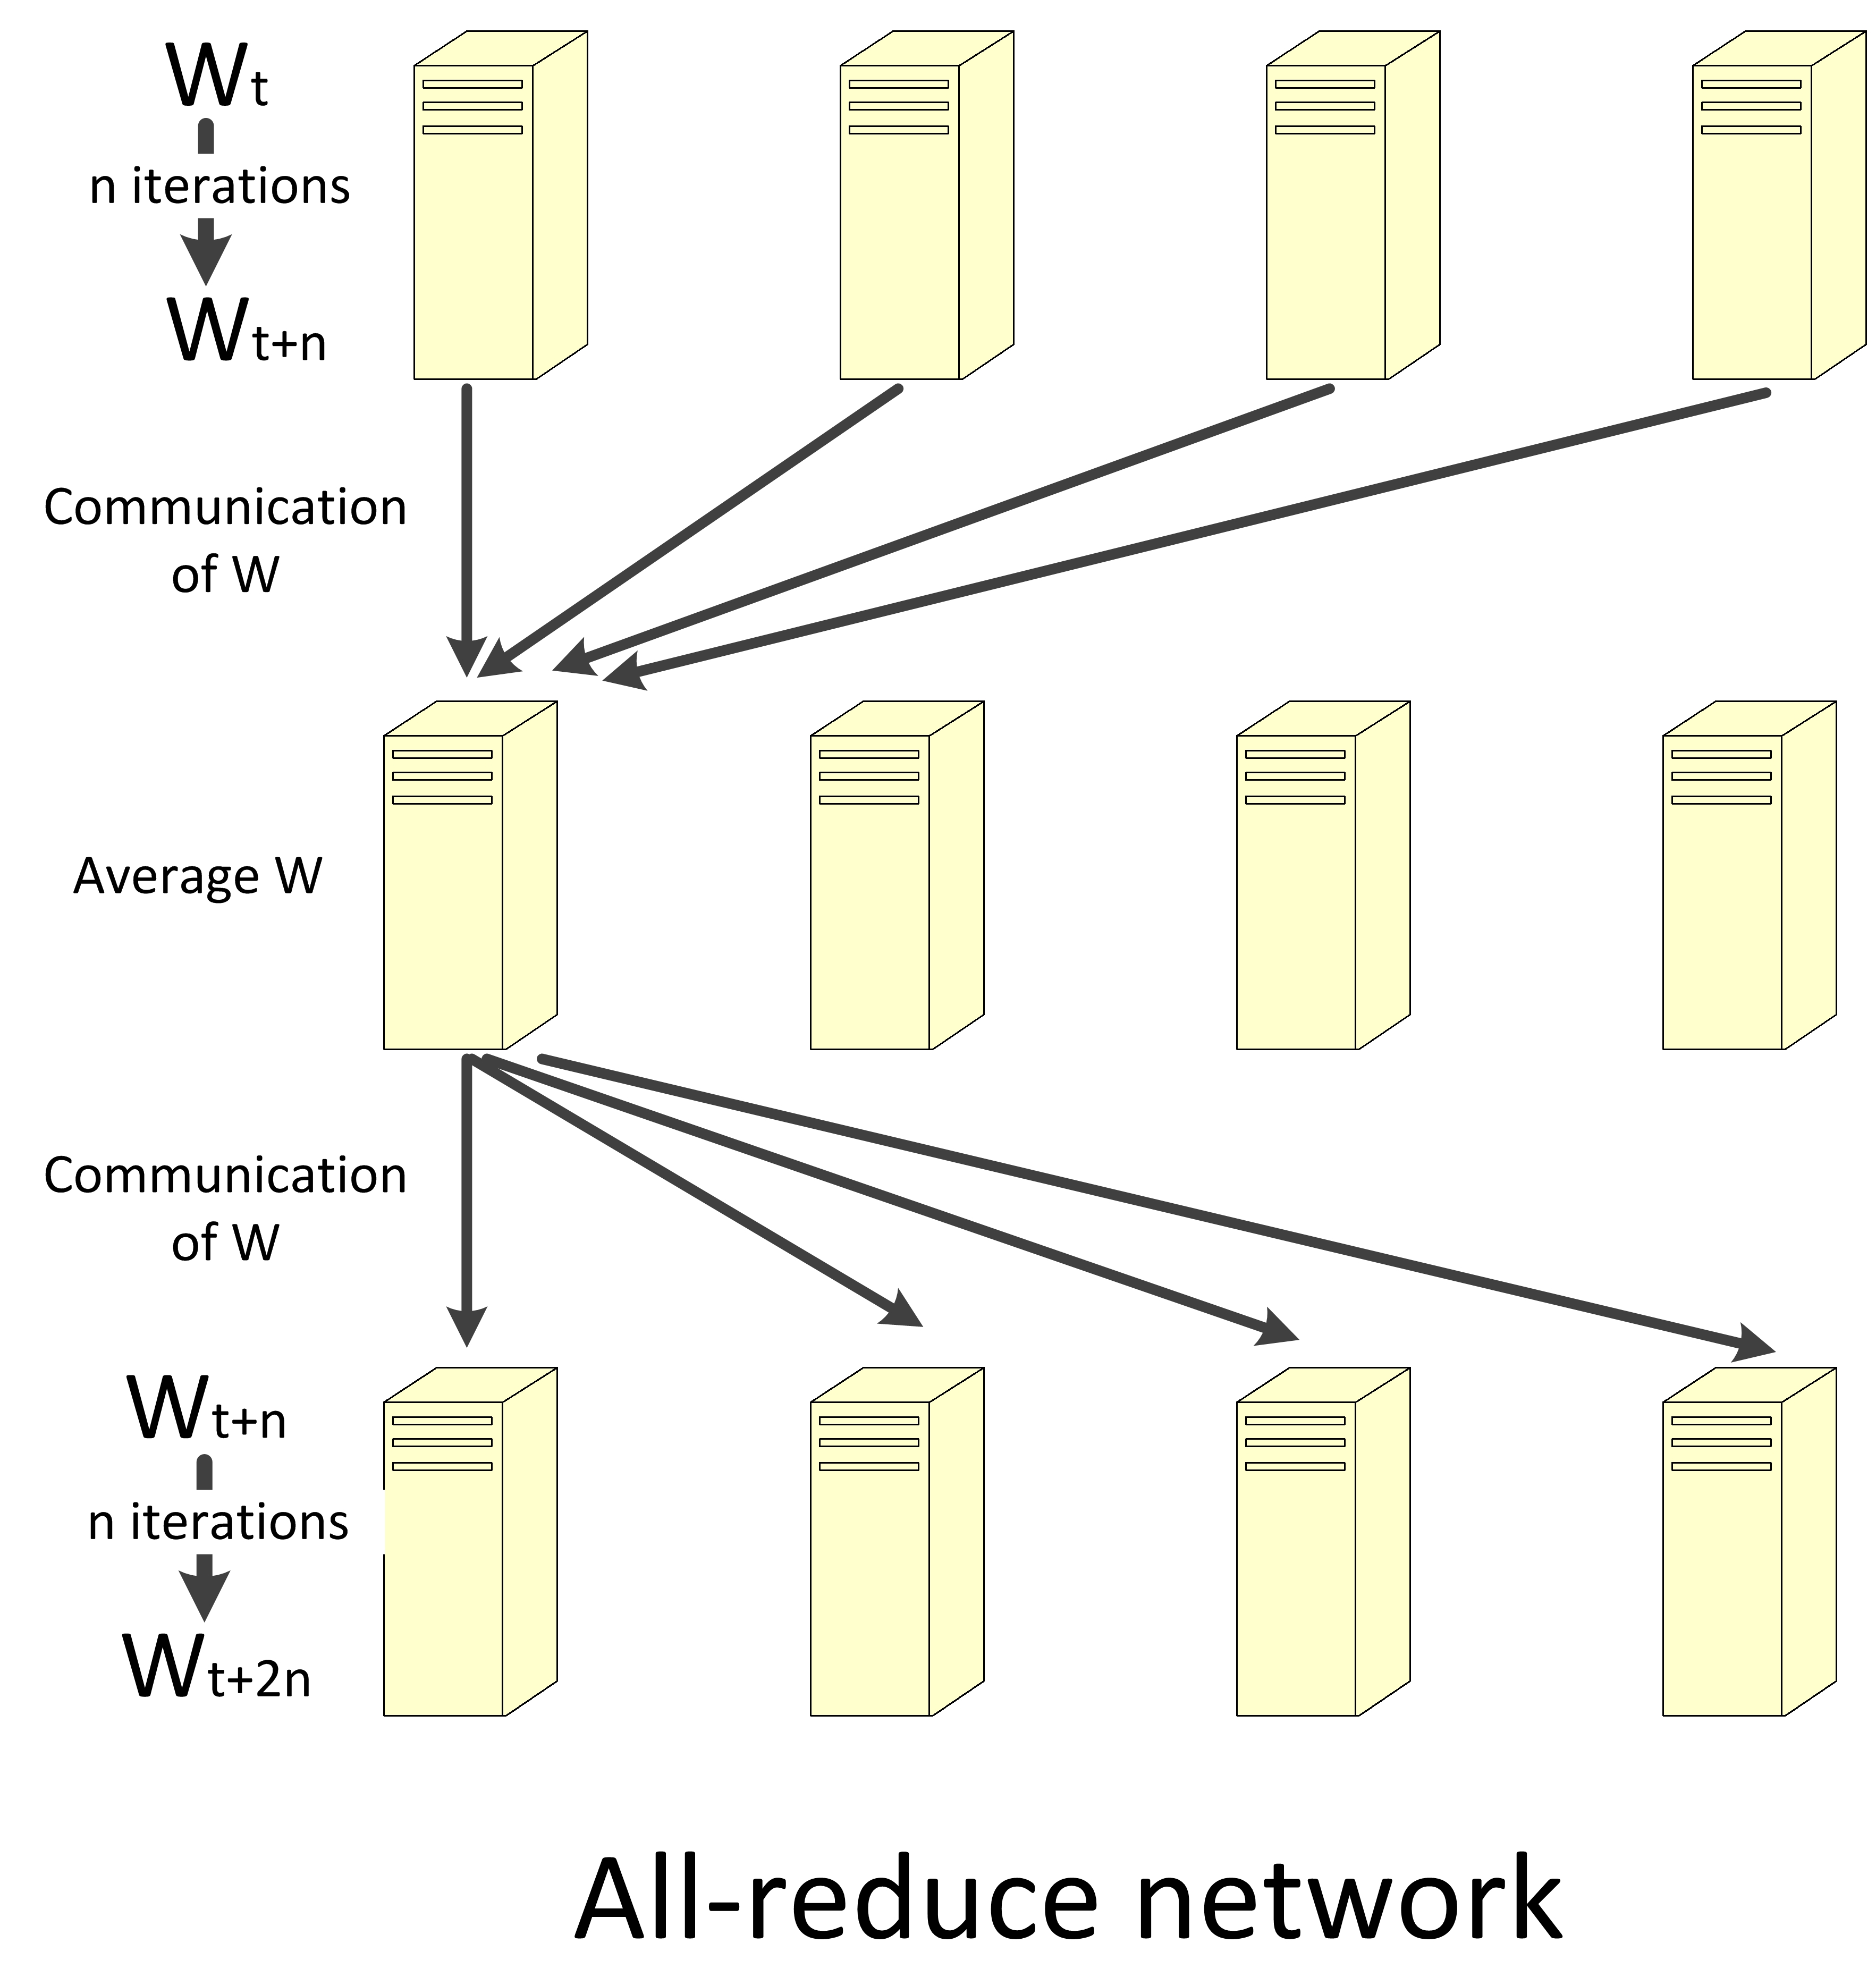
\includegraphics[width=0.5\textwidth]{allreduce.jpg}
    \caption{All-reduce network}
\end{figure}
\subsection{Butterfly Mixing}
 
Zhao and Canny (2012) proposed the butterfly mixing strategy. The butterfly mixing can reduce the communication for each iteartion: one node would only send and recieve message from one other node. But their communication orders are changed so that information for the whole network still can be spread to all nodes. Fig.~2 is an example of butterfly mixing with 4 nodes. The communication of butterfly mixing is bounded by the lantency. And butterfly mixing only require once communication to collect and average the weight, it does not need to send the averaged weight. Thus, the butterfly mixing has much less communication amount than all-reduce strategy. However, one node at butterfly mixing network only collect partial information from the network, its averaged weight can only reflect the information from two nodes. It takes $log(number of nodes)$ communication times to spread the message to the whole network. Thus, the converge speed of butterfly mixing is slower than all-reduce strategy. 
\begin{figure}[h!]
  
  \centering
    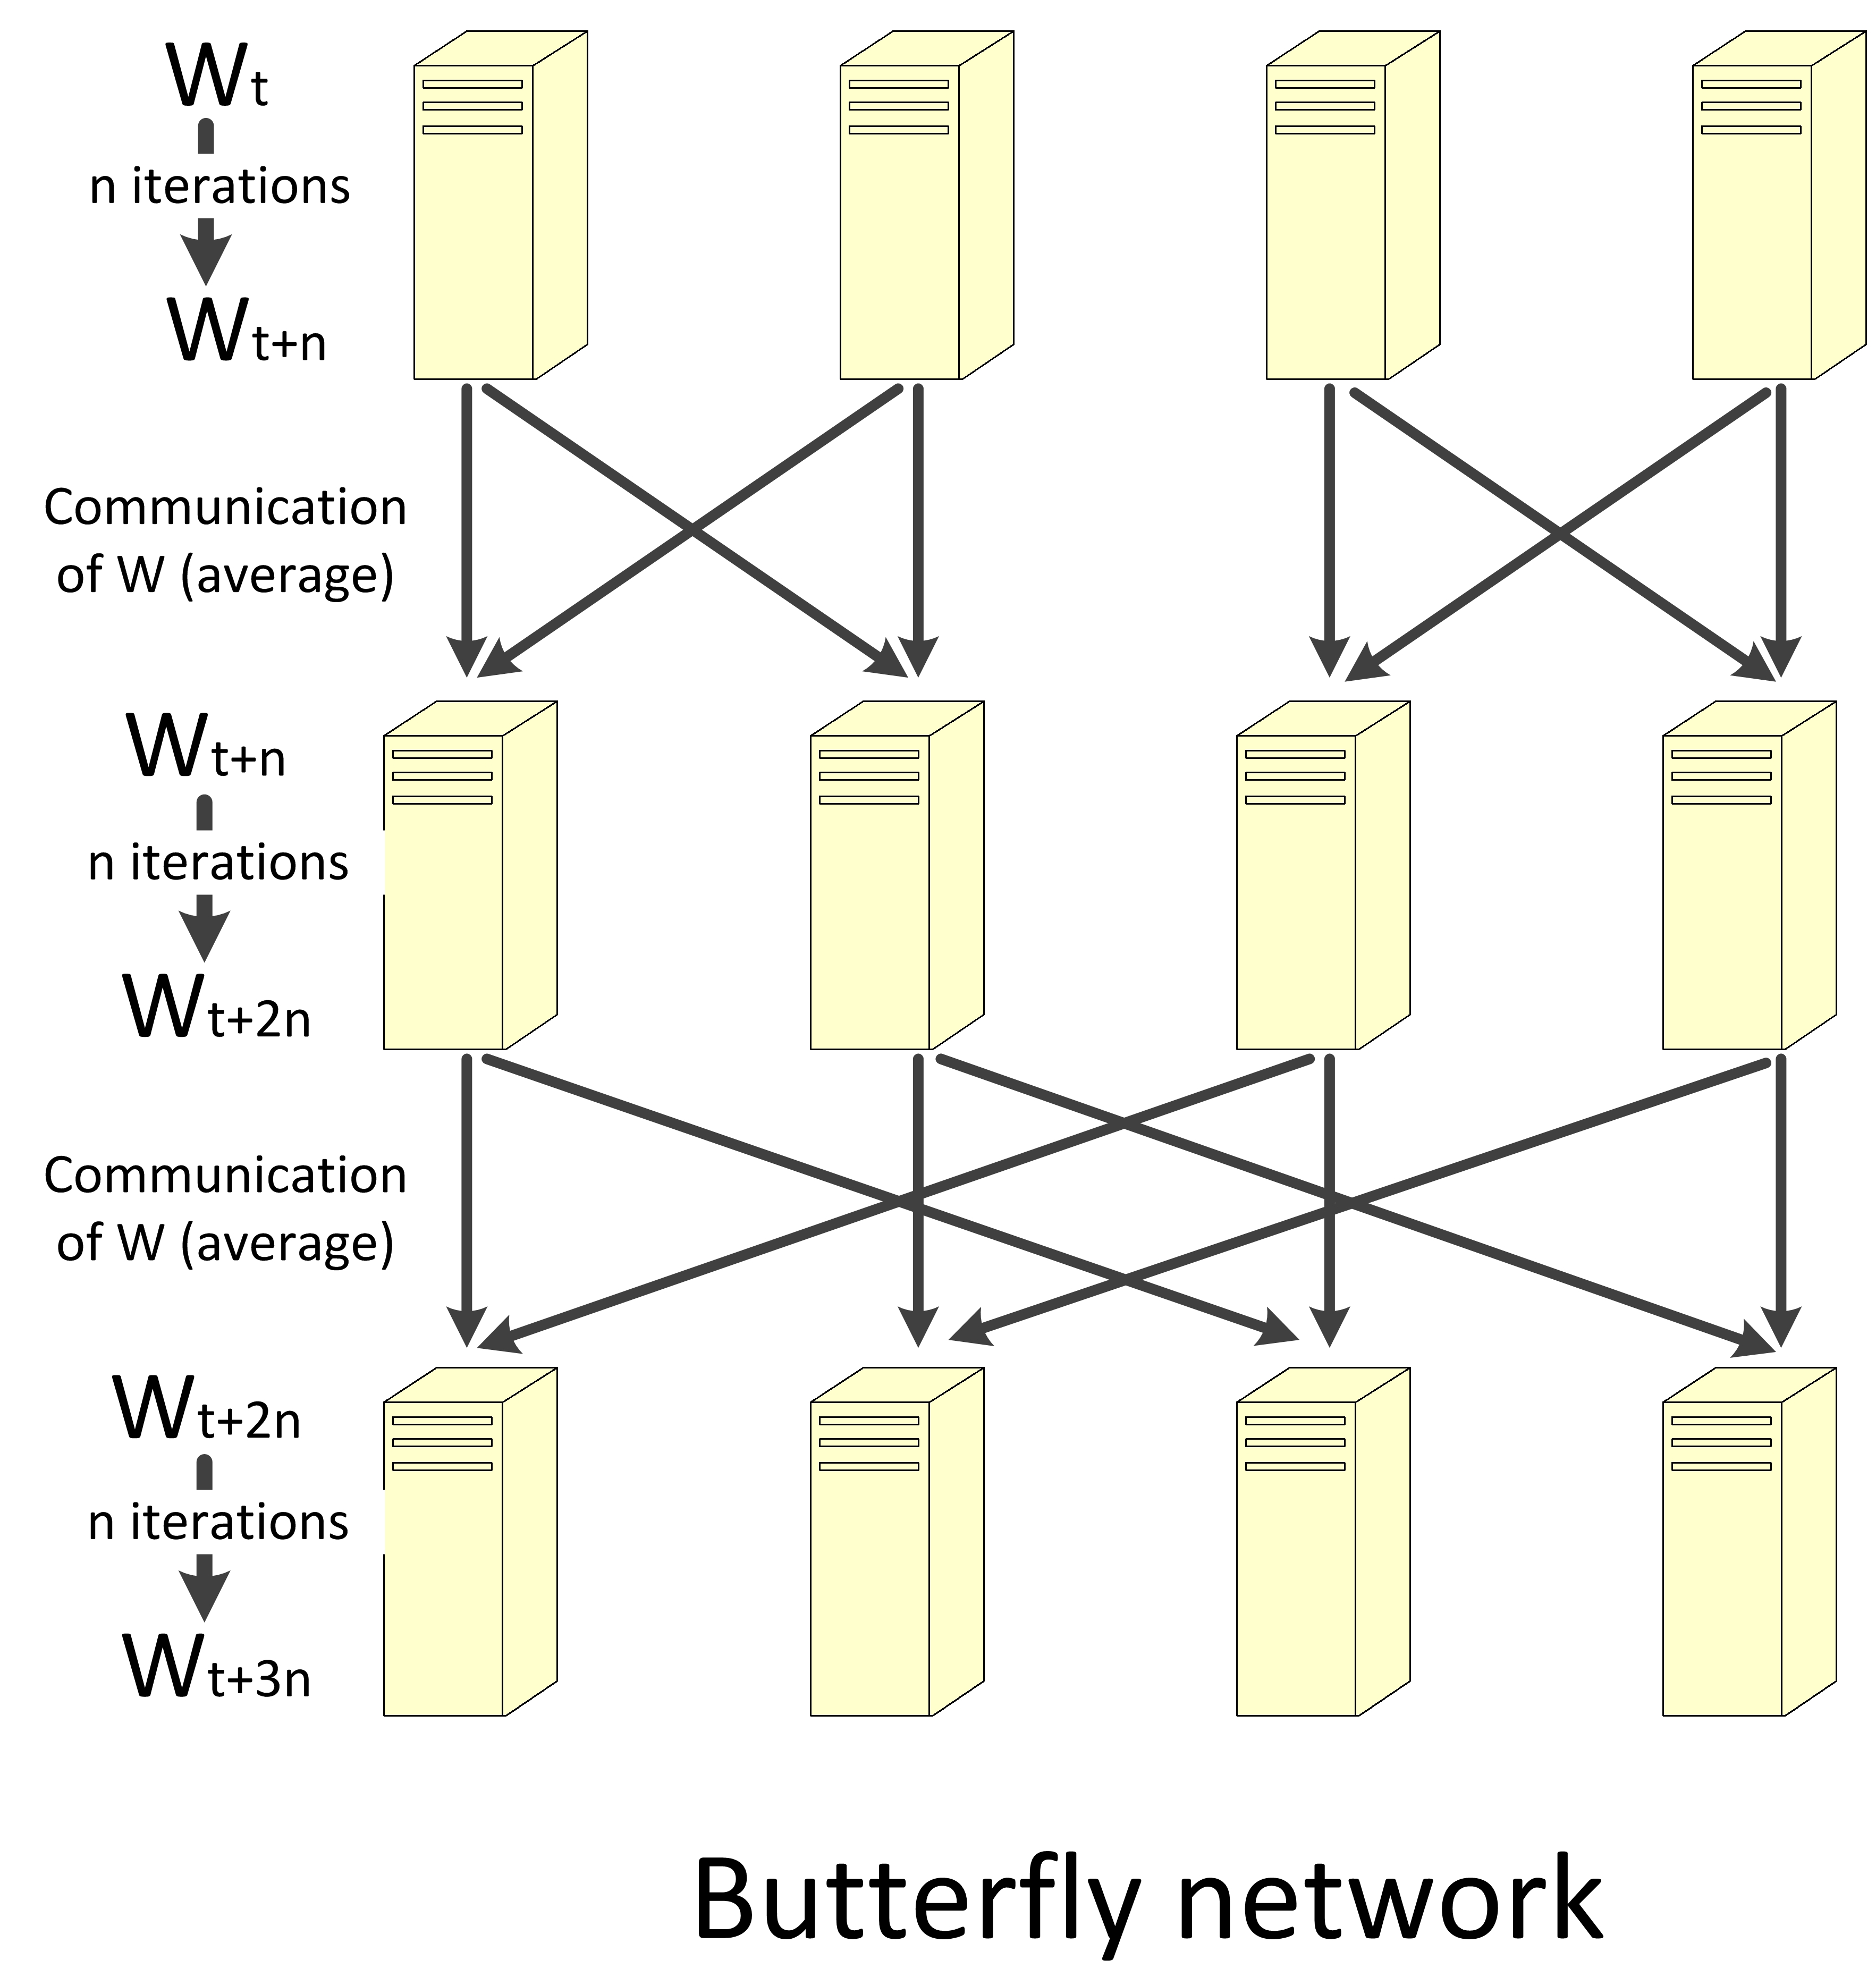
\includegraphics[width=0.5\textwidth]{butterfly.jpg}
    \caption{Butterfly mixing network.}
\end{figure}

\subsection{Ring \& Hopping Ring Reduce}

Each node in ring reduce network would send message to the next node, and receive message from the previous node, see Fig.~3. Similar as the butterfly mixing, ring network is bounded by the network latency. Ring network also only requires once communication to send and collect the weight. However, the ring network requires $number of nodes$ communication times to spread the message thoughout the whole network. Thus, the converge speed of ring network is the slowest among these three networks. 
\begin{figure}[h!]
  
  \centering
    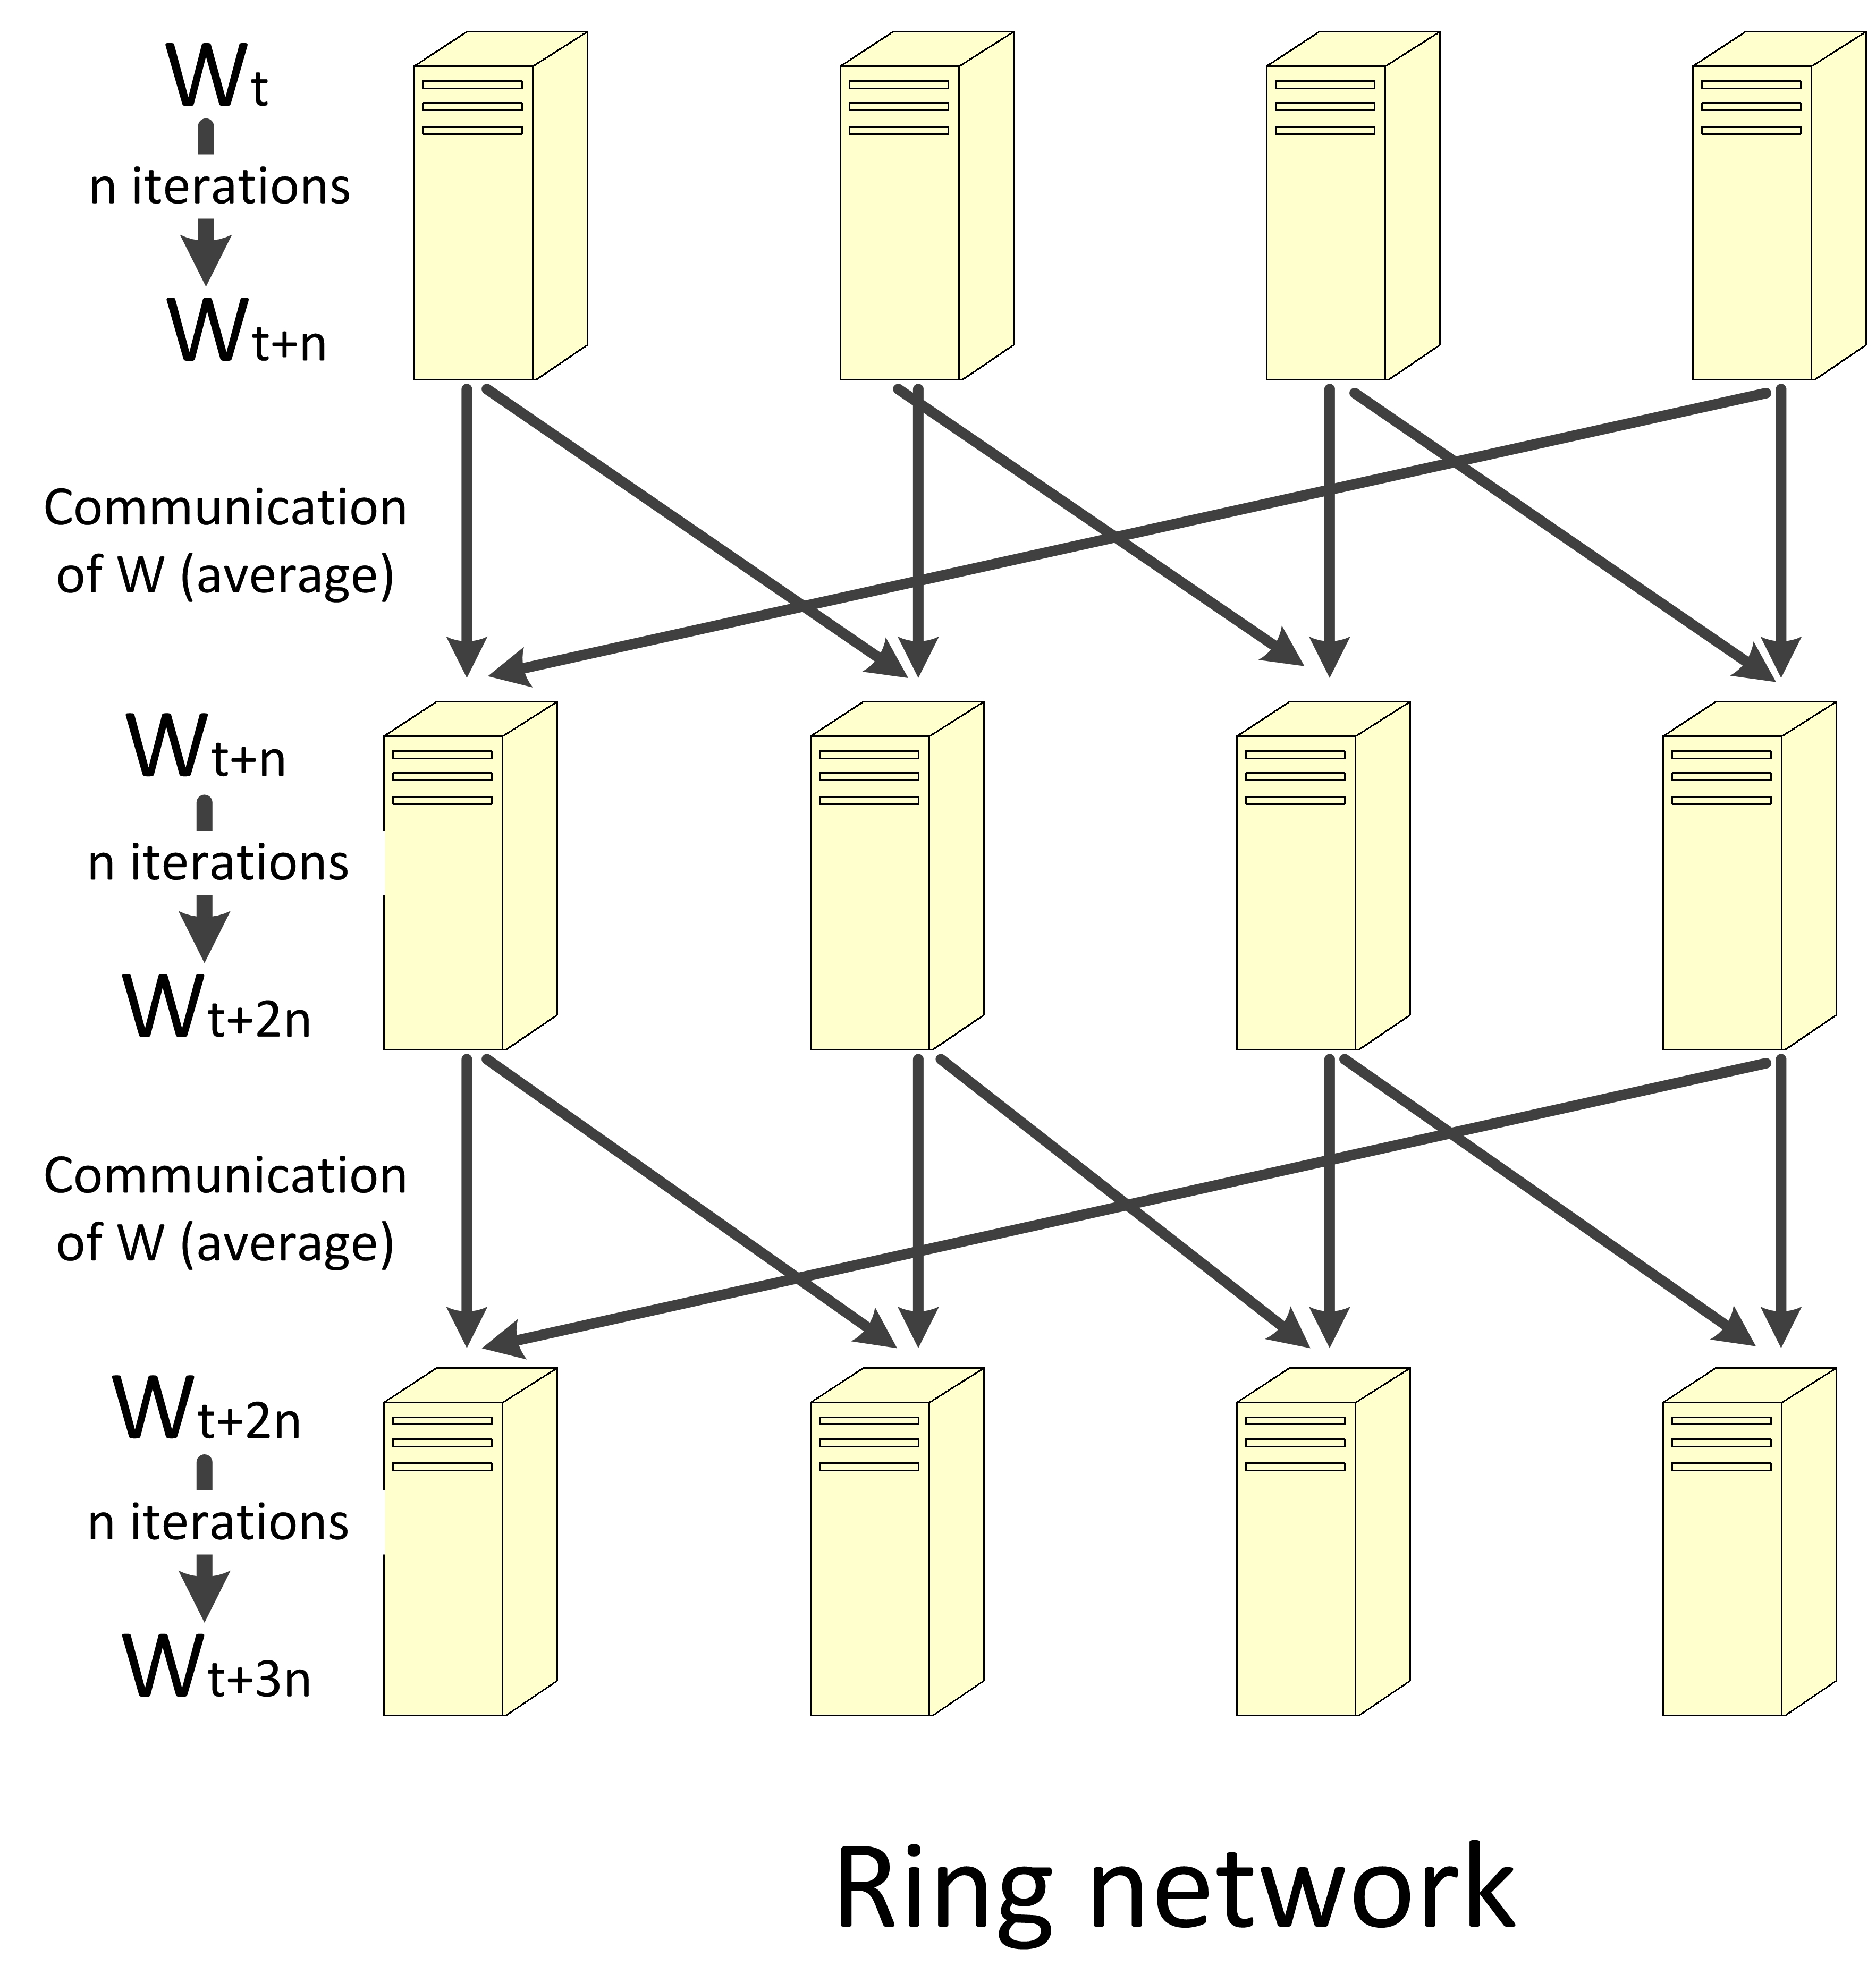
\includegraphics[width=0.5\textwidth]{ring.jpg}
    \caption{Ring network}
\end{figure}
\section{Natural Gradient for Model Update}

\section{Experimental Results}
\subsection{Reduce Frequency}

\subsection{Reduce type}

\subsection{Scaling factor}

\section{Conclusion}


\section{Acknowledgements}
We would like to thank Forrest Iandola for helpful suggestion.

% References should be produced using the bibtex program from suitable
% BiBTeX files (here: strings, refs, manuals). The IEEEbib.bst bibliography
% style file from IEEE produces unsorted bibliography list.
% -------------------------------------------------------------------------
\bibliographystyle{IEEEbib}
\bibliography{report}

\end{document}
